% Chapter 3

\chapter{Iterative Techniques for Mixed-Integer Linear Programming Problems } % Main chapter title

\label{Chapter3} % For referencing the chapter elsewhere, use \ref{Chapter2} 
%%%%%%%%%%%%%%%%%%%%%%%%%%%%%%%%%%%%%%%%%%%%%%%%%%%%%%%%%%%%%%%%%%%%%%%%%%%%%%%

%%%%%%%%%%%%%%%%%%%%%%%%%%%%%%%%%%%%%%%%%%%%%%%%%%%%%%%%%%%%%%%%%%%%%%%%%%%%%%%
Quantum computers are not mature enough to solve real-world problems. For instance, the embedding of a QUBO problem into the architecture of a quantum annealer impose a big constraint in the number of variables our problem can have. For this reason, a \textit{hybrid quantum-classical} (HQC) approach is currently the best method one can use to tackle large-scale problems, by combining quantum and classical solvers.\\\\
The aim of HQC approaches is to decompose a problem into a \textit{sub-problem(s)} (SP(s)) and \textit{master problem} (MP), so hopefully one of these problems is suitable for a quantum computer, e.g., a quantum annealer would receive a QUBO problem or a problem that can be cast into it. On the other hand, the rest of the problems are solved by the classical solver using cutting-edge algorithms. The MP and SP(s) are solved interactively until a given stopping criterion is satisfied. \\\\
There are classical systematic approaches that converge such as the Benders decomposition algorithm\,\cite{Sahinidis1991BDConvergence} meanwhile others heuristic approaches do not guarantee the optimal solution but they require less computational resources to find a sub-optimal solution by exploring the configuration space according to some criteria.\\\\
In this chapter, we describe the general formulation of a mixed-integer linear programming problem, then we present the most relevant results of dual dynamic programming theory which is the underlying theory of problem decomposition to finally show a quantum-classical benders decomposition protocol\,\cite{Zhao2021HybridProgramming}, an heuristic quantum-classical protocol\,\cite{Ding2019ImplementationDesign} and another version inspired on it.
%%%%%%%%%%%%%%%%%%%%%%%%%%%%%%%%%%%%%%%%%%%%%%%%%%%%%%%%%%%%%%
% MILP
%%%%%%%%%%%%%%%%%%%%%%%%%%%%%%%%%%%%%%%%%%%%%%%%%%%%%%%%%%%%%%
\section{Mixed-Integer Linear Programming}
In the present work, we are interested in mixed-integer linear programming (MILP) problems because they appear in a wide range of real-world applications and they represent the mathematical formulation of TEP problems. More precisely, TEP problems contains real variables but these variables are often converted to integer values to solve the problem.\\\\
The mathematical formulation of MILP problems is
\begin{mini}|l|
	{\textbf{x}}{f(\textbf{x})}{\label{eq: MILP}}{}{\left[f: \mathbb{R}^{n} \rightarrow \mathbb{R}\right]}
	\addConstraint{h(\textbf{x})}{=0,}{\left[h: \mathbb{R}^{n} \rightarrow \mathbb{R}^{m}\right]}
	\addConstraint{g(\textbf{x})}{\leq 0,\quad}{\left[g: \mathbb{R}^{n} \rightarrow \mathbb{R}^{p}\right],}
\end{mini}
where $m$ and $p$ are the number of equality and inequality constraints, respectively.\\\\
TEP problems scale badly as the problem size grows. Thus, they cannot be solved at the desired resolution by nowadays classical computers with solvers such as Gurobi\,\cite{gurobi}, CPLEX\,\cite{cplex2009v12} or cbc\,\cite{cbc}. There are already benchmarks comparing classical solvers and quantum annealers for energy problems where the best of these solvers -- Gurobi -- exceed the run-time, see Ref.\,\cite{Fernandez-Campoamor2021CommunityAnnealing}.\textbf{COMENTARIO ORIOL}\\\\
%%%%%%%%%%%%%%%%%%%%%%%%%%%%%%%%%%%%%%%%%%%%%%%%%%%%%%%%%%%%%%%%%%
% Classical Benders Decomposition
%%%%%%%%%%%%%
\section{Classical Benders Decomposition}
The main idea behind classical \textit{Benders decomposition} (BD) -- also known as \textit{dual dynamic programming} (DDP) -- is to decompose the primal problem into a master problem and a sub-problem(s) once the complicated variables are detected. In the following sections we introduce some of the remarkable results of dual dynamic programming, for a deeper understanding see\,\cite{bierlaire2018}.
%%%%%%%%%%%%%
\subsection{Complicated Variables}
We can consider a decision variable to be complicated if the decision variable is involved in most of the constraints or the decision variable produce non-convex optimization problems. 
\begin{definition}{Complicated variables}{}
Those variables that allow us to split the original problem into sub-problem(s) when they are fixed. 
\end{definition}
After splitting the original problem, the master problem is a relaxed version of the original problem, which has the complicated variables with their constraints, i.e., relaxed optimization problem. The global minimum is guarantee if and only if the objective function as function of the complicated variables is a convex envelope.\\\\
For this reason, BD decompose the general problem \eqref{eq: MILP} into a MP with integer variables and a SP so that a clever re-arrange of the variables allow us to fixed complicated variables the MP and send these complicated variables as fixed for the sub-problem, then both problems are solved interactively until a stopping criterion is satisfied. The convergence of BD\,\cite{Sahinidis1991BDConvergence} guarantees that we can satisfy an arbitrary threshold value after a number of iterations. 
%%%%%%%%%%%%%%%%%%%%%%%%%%%%%%
\subsection{Dual Dynamic Programming}
We can relax the primal problem by associating a penalty to each of them,
\begin{equation}
    \lambda\in\mathbb{R}^{m}\,\, \text{and} \quad \mu\in\mathbb{R}^{p},
\end{equation}
also known as Lagrange multipliers or dual variables. Then the Lagrangian of the primal problem is
\begin{equation}
    \mathcal{L}(\textbf{x}, \lambda, \mu) = f(\textbf{x}) + \lambda^{\intercal}h(\textbf{x}) + \mu^{\intercal}g(\textbf{x}).
\end{equation}
\begin{definition}{Dual function}{}
The dual function, $q: \left[\mathbb{R}^{m+p}\rightarrow\mathbb{R}\right]$, maps the set of parameters $\lambda$ and $\mu$ to a minimization problem
\begin{equation}
    q(\lambda, \mu) = \min_{x\in\mathbb{R}^{n}}\mathcal{L}(\textbf{x}, \lambda, \mu),
\end{equation}
where $m$ and $p$ are the number of equality and inequality constraints, respectively and
\begin{equation}
    \lambda\in\mathbb{R}^{m}\,\, \text{and} \quad \mu\in\mathbb{R}^{p},
\end{equation}
are the penalty parameters.
\end{definition}
Notice that the dual function is an unsconstrained problem because all the constraints have been move into the Lagrangian.
Consider the MILP problem \eqref{eq: MILP}. In that problem, the inequality constraint $g(\textbf{x})\leq 0$ is violated if $g(\textbf{x})>0$. To take into account this in the cost function we need to introduce a positive cost, so $\mu^{\intercal}g(\textbf{x})>0$ which implies $\mu^{\intercal}$ has positive coefficients.
\begin{theorem}{}{}
The dual of a linear optimization problem is another linear optimization problem.
\end{theorem}
\begin{theorem}{}{}
The dual of the dual is the primal.
\end{theorem}
\begin{theorem}{}{}
Suppose that $\textbf{x}^{*}$ is an optimal solution of the primal. Then,
\begin{equation}
    q(\lambda, \mu) \leq f(\textbf{x}^{*})
\end{equation}
is a lower bound on the optimal value of the primal problem, for
\begin{equation}
    \lambda\in\mathbb{R}^{m}\,\, \text{and} \quad \mu\in\mathbb{R}^{p}.
\end{equation}
\end{theorem}
\begin{proof}
\begin{align}
    q(\lambda, \mu) = \min_{\textbf{x}\in \mathbb{R}^{n}} \mathcal{L}(\textbf{x}, \lambda, \mu) \leq \mathcal{L}(\textbf{x}^{*}, \lambda, \mu) = f(\textbf{x}^{*}) + \lambda^{\intercal}h(\textbf{x}^{*}) + \mu^{\intercal}g(\textbf{x}^{*}) \leq f(\textbf{x}^{*})
\end{align}
\end{proof}
\begin{corollary}{}{}
  In particular, of $\textbf{x}^{*}$ is an optimal solution of the primal and $\textbf{x}$ is a feasible solution of the primal, then
  \begin{equation}
      \underbrace{q({\lambda,\mu})}_{\text{Lower Bound}} \leq f(\textbf{x}^{*}) \leq \underbrace{f(\textbf{x})}_{\text{Upper Bound}}
  \end{equation}
\end{corollary}
We want to find the best possible lower bound by solving the following optimization problem
\begin{maxi}|l|
	{\lambda, \mu}{q(\lambda, \mu)}{\label{eq: Abstract_Dual}}{}{\left[g: \mathbb{R}^{m+p} \rightarrow \mathbb{R}\right]}
	\addConstraint{\mu}{\geq 0}{}
	\addConstraint{(\lambda, \mu)}{}{\in \{\lambda, \mu \,/\, q(\lambda, \mu) > - \infty \},}.
\end{maxi}
Notice that we are choosing the penalties in such a way that te dual problem is bounded.
\begin{theorem}{Weak Duality}{}
If $\textbf{x}^{*}$ is the optimal solution of the primal, and $\lambda^{*}, \mu^{*}$ is the optimal solution of the dual, then
\begin{equation}
    q(\lambda^{*}, \mu^{*}) \leq f(\textbf{x}^{*})
\end{equation}
\end{theorem}
\begin{theorem}{Strong Duality}{}
If $\textbf{x}^{*}$ is the optimal solution of the primal, and $\lambda^{*}, \mu^{*}$ is the optimal solution of the dual, then
\begin{equation}
    q(\lambda^{*}, \mu^{*}) = f(\textbf{x}^{*})
\end{equation}
\end{theorem}
\begin{corollary}{}{}
If one either the primal problem of the dual problem is unbounded, then both problems are unbounded.
\end{corollary}
\begin{proof}
If the primal is unbounded, then
\begin{equation}
    q(\lambda^{*}, \mu^{*}) \leq \infty
\end{equation}
which implies the dual problem is unbounded. Analogously, if the dual problem is unbounded, then the primal problemis unbounded too.
\end{proof}
\begin{corollary}{}{}
If there exist $\textbf{x}^{*},\lambda^{*}\,\text{and}\, \mu^{*}$ such that,
\begin{equation}
    q(\lambda^{*}, \mu^{*}) = f(\textbf{x}^{*})
\end{equation}
then they are optimal.
\end{corollary}
\begin{proof}
Consider a feasible solution of the primal problem, $\textbf{x}$ and a feasible solution of the dual problem $(\lambda, \mu)$, then
\begin{equation}
    f(\textbf{x}) \geq q(\lambda^{*}, \mu^{*}) = f(\textbf{x}^{*}) \geq q(\lambda, \mu)
\end{equation}
\end{proof}
%%%%%%%%%%%%%%
\begin{figure}[H]
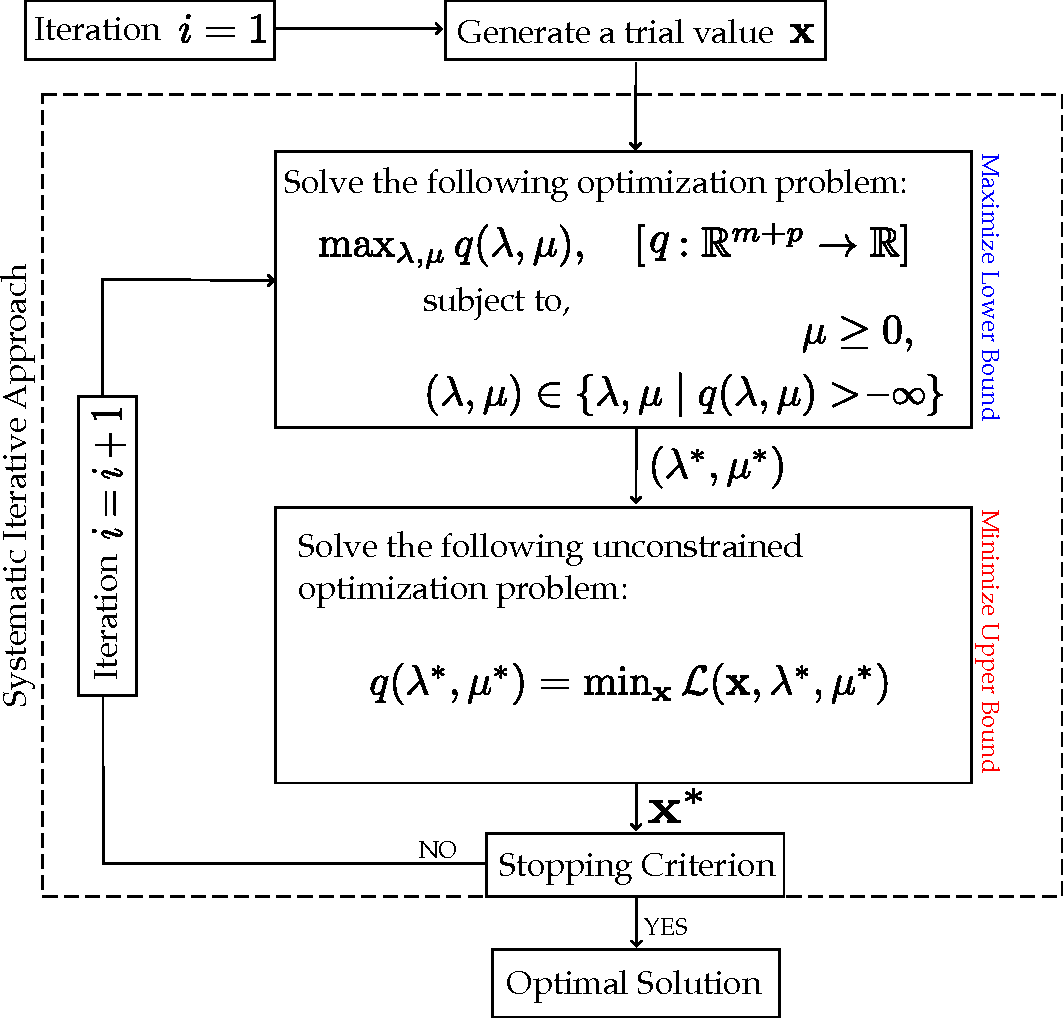
\includegraphics[width=0.8\textwidth]{Figures/BDScheme.pdf} 
\caption{Benders decomposition scheme.}
\label{fig:BDScheme}
\end{figure}
The solution of the master problem, $f(\textbf{x)}$, generates a lower bound, meanwhile the solution of the sub-problem, $q(\lambda, \mu)$, generate an upper bound. Both problems are solved interactively until lower and upper bound satisfy a given stopping criterion $|f(\textbf{x}) - q(\lambda, \mu)| = \epsilon$.\\\\
\subsection{Benders' Decomposition: An Illustrative Example}
As an example, consider a general expansion planning problem with cost function given by
\begin{equation}
    \min_{x_{3},g_{1}(h),g_{2}(h),g_{3}(h)}\underbrace{30000x_{3}}_{\text{Investment Cost}} + \underbrace{\sum_{h}10g_{1}(h)+20g_{2}(h) + 5g_{3}(h)}_{\text{Operational Cost}}\\ 
\end{equation}
subject to a set of constraints,
\begin{align}
    0 \leq g_{1}(h) \leq 100, \quad \forall\,h\\
    0 \leq g_{1}(h) \leq 200, \quad \forall\,h\\
    \underbrace{0 \leq g_{2}(h) \leq x_{3}}_{\text{Linking Constraint}}, \quad \forall\,h \\
    D(h) = g_{1}(h) + g_{2}(h) + g_{3}(h), \quad \forall\,h \\
    x_{3} \geq 0
\end{align}
where $x_{3}$ represent the decision of creating a new element $g_{3}$, $h$ represents the snapshot considered and $D(h)$ represents a demand to be fulfilled by the elements $\{g_{j}\}$ at snapshot $h$. Notice that if we just minimize the investment cost, then $x_{3}$ would be set to zero despite the operational cost of the element $g_{3}$ is cheaper than the other elements. Moreover, notice that if we consider a large set of snapshots $h$, then the operational cost is the dominant term. Analogously, for a short set of snapshots the investment cost is the dominant term of the total cost function. In summary, extremal solutions lead to a high value of cost function in one of this ways
\begin{itemize}
    \item \textbf{Underinvestment} leads to a high value of the total cost function because the system is not able to fulfill the demand $D(h)$.
    \item \textbf{Overinvestment} leads to a high value of the total cost function despite it fulfill the demand. Intuitively, we are creating more elements $\{g_{j}\}$ than we need. Usually there is an upper bound due to capital budget.
\end{itemize}
The optimization problem is a trade-off between operational cost and investment cost where the optimal solution minimize the investment cost and operational cost fulfilling at the same time the constraints of the problem.
%%%%%%%%%%%%%%%%%%%%%%%%%%%%%%%%%%%%%%%%%%%%%%
 For instance, suppose that the decision variable $x_{3}$ of the previous cost function is a complicated variable, it is involved in a linking constraint. Fixing that variable to a feasible value and considering a single snapshot $h=1$ would allow us to write the master problem as,
\begin{equation}
    \min_{x_{3}^{(i)}, \alpha^{(i)}} 30000x_{3}^{(i)} + \alpha^{(i)}
\end{equation}
subject to
\begin{align}
    x_{3}^{(i)} \geq 0 \\
    \alpha^{(i)} \geq \alpha^{(\text{down})}
\end{align}
where $\alpha^{(\text{down})}$ is a lower bound of the master problem and $(i)$ indicate the interation counter. Once the master problem is optimised we fix $x_{3}^{(\text{fixed})}$ to the optimal value found in the master problem and write the sub-problem as
\begin{equation}
    \min_{g_{1}^{(i)}(1), g_{2}^{(i)}(1), g_{3}^{(i)}(1)} 10g_{1}^{(i)}(1)+20g_{2}^{(i)}(1) + 5g_{3}^{(i)}(1)
\end{equation}
subject to
\begin{align}
    0 \leq g_{1}^{(i)}(1) \leq 100 \quad :\pi^{(i)} \\
    0 \leq g_{1}^{(i)}(1) \leq 200 \quad :\mu^{(i)} \\
    0 \leq g_{2}^{(i)}(1) \leq x_{3}^{((i))(\text{fixed})} \quad :\sigma^{(i)} \\
    D(h) = g_{1}^{(i)}(1) + g_{2}^{(i)}(1) + g_{3}^{(i)}(1) \quad :\gamma^{(i)}
\end{align}
where $\pi^{(i)}$, $\mu^{(i)}$, $\sigma^{(i)}$ and $\gamma^{(i)}$ are the dual variables associated with each constraint. The sub-problem find the optimal configuration $\{g_{j}(1)\}$ for a given fixed value $x_{3}^{(\text{fixed})}$, then it updates the master problem parameter $\alpha^{(i)}$ according to
\begin{equation}
    \min_{x_{3}^{(i)}. \alpha^{(i)}} 30000x_{3}^{(i)} + \alpha^{(i)}
\end{equation}
subject to
\begin{align}
    x_{3}^{(i)} \geq 0 \\
    \alpha^{(i)} \geq \alpha^{(\text{down})}\\
    \alpha^{(i)} \geq -\
\end{align}
The last constraint represents the dual objective function of the sub-problem in iteration $i$. In other words, it is a function of $x_{3}$. $k$ represent the previous Benders Cuts (it is necessary?). We are following the systematic iterative process of figure \ref{fig:BDScheme}.
\begin{figure}[H]
\centering
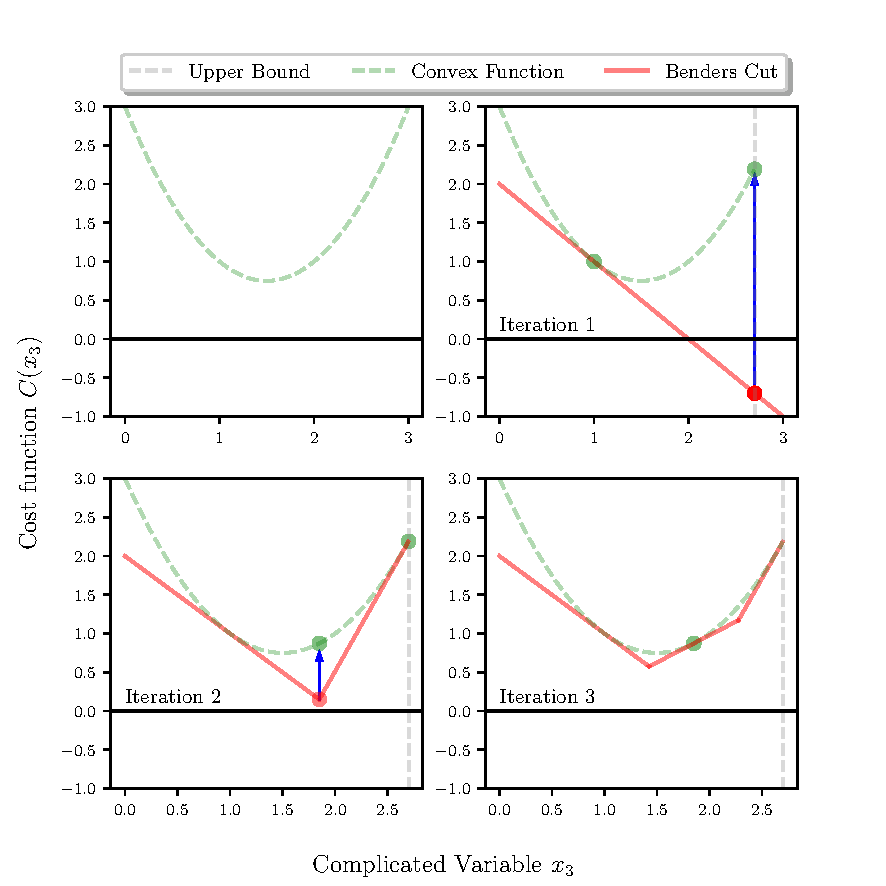
\includegraphics[width=\textwidth]{Figures/BenderIlustration.pdf} 
\caption{Graphical representation of CBD protocol for a single complicated variable in an arbitrary convex function.}
\label{fig:BDIlustration}
\end{figure}
%%%%%%%%%%%%%%%%%%%%%%%%%%%%%%%%%%%%%%%%%%%%%%%%%%%%%%%%%%%%%%%%%%%%%%%%%%%%%%%
% QA + SA
%%%%%%%%%%%%%%%%%%%%%%%%%%%%%%%%%%%%%%%%%%%%%%%%%%%%%%%%%%%%%%%%%%%%%%%%%%%%%%%
\section{Hybrid quantum-classical algorithms}
In Appx.\,\ref{AppendixB}, we show the foundations of \textit{simulated annealing} algorithm (SA) and solve a travelling salesman problem to illustrate it. A simulated annealing algorithm does not guarantee to get the optimal solution but the results we can get with a clever annealing schedule are good enough in accuracy and time. Analogously with a quantum annealing algorithm. In this section, we show how the decomposition of a QUBO problem allow us to use both quantum and classical solvers, where the classical solvers relaxed the original problem so that it can be tackled by the quantum solver.
%%%%%%%%%%%%%%%%%%%%%%%%%%%%%%%%%%%%%%%%%%%%%%%%%%%%%%%%%%%%%%%%%%%%%%%%%%%%%%%
\subsection{Quantum Benders' Decomposition: Single Cuts}
In this section, we show the protocol of quantum Benders' decomposition for single cuts. A multi-cuts quantum Benders' decomposition algorithm with an application to power energy sector is online \,\cite{Paterakis2021HybridApplication}.
\begin{figure}[H]
\centering
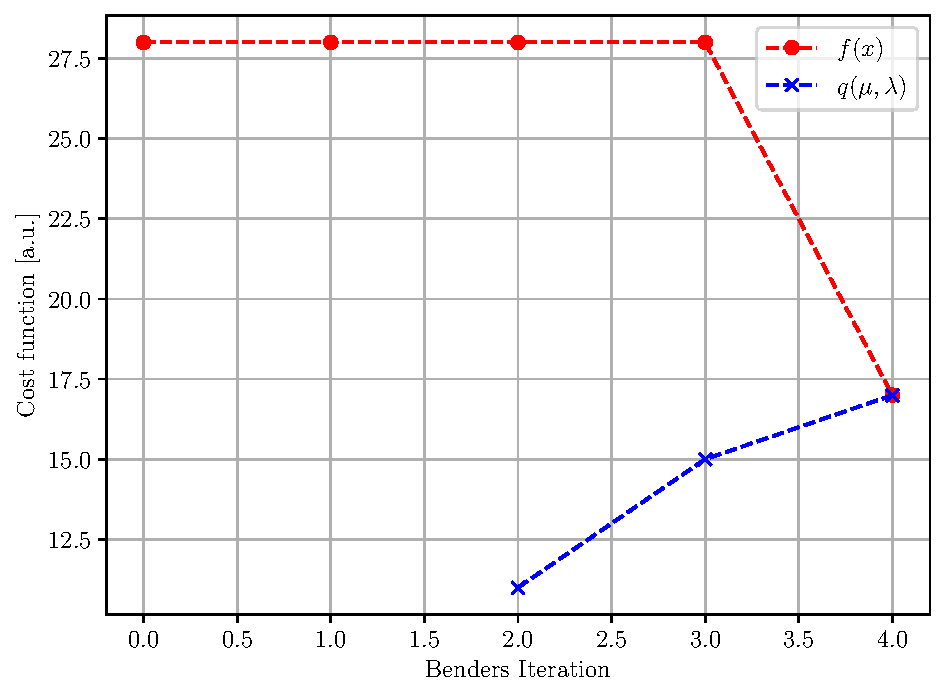
\includegraphics[width=\textwidth]{Figures/BD_Convergence.pdf} 
\caption{Benders Convergence\,\cite{Zhao2021HybridProgramming}.}
\label{fig:BD_Convergence}
\end{figure}
%%%%%%%%%%%%%%%%%%%%%%%%%%
\subsection{Heuristic Protocols}
As stated before, heuristic approaches do not guarantee to arrive at the optimal solution. However, these methods explore the configuration space in such a way that we do not get stuck in a local minimums. For a limited amount of computational resources and time, the solution that an heuristic approach can achieve is sub-optimal. Generally, these methods are better than a brute-force method when the problem is large enough so that there are not computational resources to solve it by getting the optimal solution.
\subsubsection{SA-QA Protocol}
We present a hybrid quantum-classical algorithm protocol based on combining SA and QA\,\cite{Ding2019ImplementationDesign} to solve the MP and SP(s), respectively.
\begin{figure}[H]
\centering
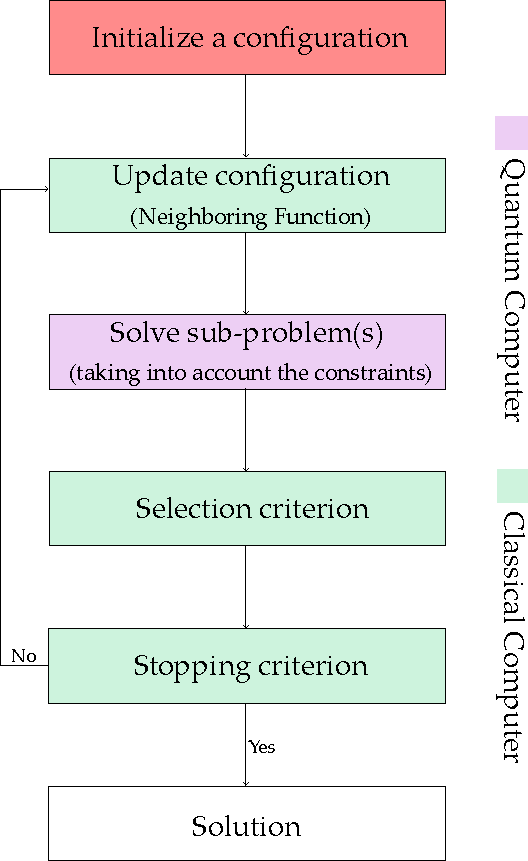
\includegraphics[width=0.45\textwidth]{Figures/SAQAProtocol_Layer 1.pdf} 
\caption{SA-QA protocol scheme.}
\label{fig:SA_QAProtocol}
\end{figure}
\begin{enumerate}
    \item Set the cost to a high value and initialize a configuration for the problem, i.e., annealing schedule, initial and final temperature, and a selection criterion.
    \item Randomly generate a new configuration by changing the values of the binary variables according to a neighboring function that generate a new configuration in one of these ways:
    \begin{enumerate}
        \item Randomly pick a binary variable with value 1 and set it to 0.
        \item Randomly pick a binary variable with value 0 and set it to 1.
        \item Randomly pick two binary variables with different values and swap them.
    \end{enumerate}
    \item Given the new configuration, solve the sub-problem(s) -- dual problems -- with a quantum annealing algorithm.
    \item Apply the selection criterion to keep or to discard the current configuration.
    \item If the selection criterion is not satisfied, repeat steps 2 to 4 until a iteration index is equal to the value set in step 1, then decrease the temperature and reset the iteration index. If the selection criterion is satisfied, outputs the current cost function value and its solution $\vec{x}$.
\end{enumerate}
Notice that the algorithm solve the master problem with a simulating annealing algorithm in a classical solver and then the sub-problem(s) -- dual problems -- with the quantum computer, more precisely with a quantum annealer. For this reason, the sub-problem(s) must have binary constraints or low integer values if we do not want to deal with discretization errors or adding a big set of slack variables.\\\\
In order to apply both simulated and quantum annealing to problems in which the master problem contains most of the binary and integer variables -- as happen with TEP problems--, we have to reconsider or adapt the previous scheme.
%%%%%%%%%%%%%%%%%%%%%%%%%%%%%%%%%%%%%%%%%%%%%%%%%%%%%%%%%%%%%%
% QA-SA Protocol
%%%%%%%%%%%%%%%%%%%%%%%%%%%%%%%%%%%%%%%%%%%%%%%%%%%%%%%%%%%%%%
\subsubsection{QA-SA Protocol}
 As stated before, our sub-problem(s) has real constraints which implies it is not a good idea to solve them with a quantum annealer. For this reason, we reverse the original protocol so that the quantum annealer tackle the master problem in which the binary and integer decision variables appear and the classical solver tackle the sub-problem(s).\\\\
In order to clarify the protocol to what has been shown in previous section we use the same notation $f(\textbf{x})$ to describe the upper bound of the primal problem and $q(\lambda)$ to describe the lower bound, where $(\lambda,\mu)$ represents the penalties of our problem, in other words, the Lagrange multipliers, and $\textbf{x}$ represent the decision variables. We are showing a heuristic approach, so the convergence is not guaranteed, in other words we are not getting the optimal values $(\textbf{x}^{*}, \lambda^{*},\mu^{*})$ that maximize the lower bound and minimize the upped bound in each iteration, instead we are optimizing the dual problem by SA algorithm and the master problem by QA, so that none of these methods guarantee the optimal solution to its combinatorial optimization problem.
\begin{figure}[H]
\centering
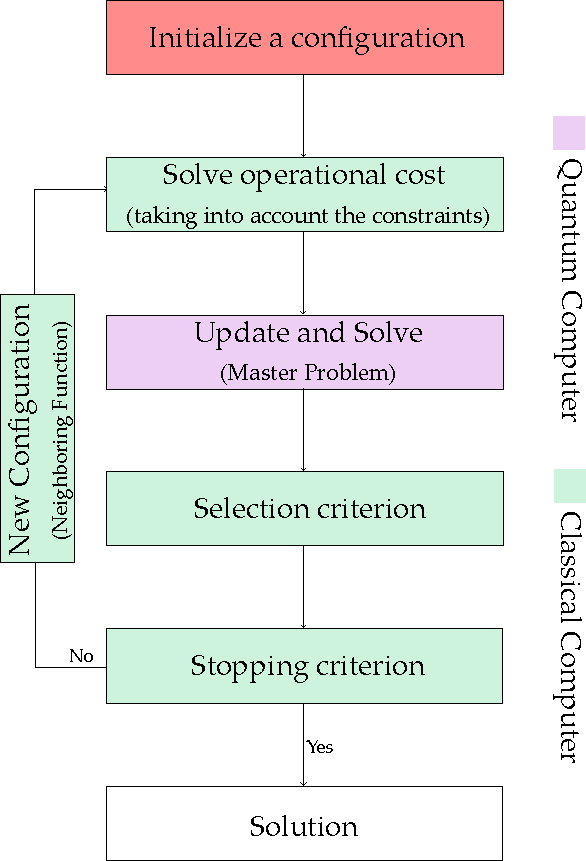
\includegraphics[width=0.5\textwidth]{Figures/QASAProtocol_Layer 1.pdf} 
\caption{QA-SA protocol scheme.}
\label{fig:QA_SAProtocol}
\end{figure}
\begin{enumerate}
    \item Set an initial feasible configuration to the primal problem $\textbf{x}$.
    \item Solve the dual problem by SA,
    \begin{maxi}|l|
	{\lambda, \mu}{q(\lambda, \mu)}{}{}{\left[g: \mathbb{R}^{m+p} \rightarrow \mathbb{R}\right]}
	\addConstraint{\mu}{\geq 0}{}
	\addConstraint{(\lambda, \mu)}{}{\in \{\lambda, \mu \,/\, q(\lambda, \mu) > - \infty \}}.
\end{maxi}
Notice that the parameters $\lambda$ and $\mu$ do not have to be the optimal parameters. SA does not guarantees to obtain the optimal solution of the dual problem.
    \item Update the master problem with $\{\lambda, \mu\}$ 
    \begin{equation}
        q(\lambda,\mu) = \min_{\textbf{x}} \mathcal{L}(\textbf{x}, \lambda, \mu)
    \end{equation}
     QA does not guarantee to obtain the optimal solution $\textbf{x}^{*}$ of the master problem.
    \item Apply the selection criterion to keep or to discard the current configuration.
    \item If stopping criterion is satisfied, then outputs the solution. Otherwise, insert the values $\textbf{x}$ of step 3 into step 2 and repeat until step 4.
\end{enumerate}



